%=====================================================================
%  UPRM Weight Gym Operations and Member-Access Platform
%  CIIC 4151 Senior Design Project
%  Overleaf-ready LaTeX source (compile with pdfLaTeX)
%
%  Condensed proposal: title page, sections I-VII, diagrams, and references.
%=====================================================================
\documentclass[11pt,letterpaper]{article}

%---------------------------- Encoding ------------------------------
\usepackage[utf8]{inputenc}     % accented characters: Mayagüez, José, Miłosz
\usepackage[T1]{fontenc}
\usepackage[english]{babel}
\IfFileExists{lmodern.sty}{\usepackage{lmodern}}{} % optional nicer font

%---------------------------- Layout --------------------------------
\usepackage[margin=1in]{geometry}
\usepackage{setspace}
\usepackage{parskip}
\usepackage{fancyhdr}
\usepackage{titlesec}

%---------------------------- Tables --------------------------------
\usepackage{array}
\usepackage{tabularx}
\usepackage{longtable}
\usepackage{booktabs}
\usepackage{ragged2e}

%---------------------------- Lists / Figures -----------------------
\usepackage{enumitem}
\usepackage{graphicx}
\usepackage{caption}

%---------------------------- Links ---------------------------------
\usepackage[hidelinks]{hyperref}
\usepackage{url}
\urlstyle{same}
\IfFileExists{xurl.sty}{\usepackage{xurl}}{} % break long URLs anywhere

%------------------- Global formatting choices ----------------------
% Sections are numbered with Roman numerals (I. INTRODUCTION ... VII. ...)
\renewcommand{\thesection}{\Roman{section}}
\titleformat{\section}{\normalfont\large\bfseries}{\thesection.}{0.6em}{\MakeUppercase}
\titleformat{\subsection}{\normalfont\normalsize\bfseries}{}{0em}{}
\titleformat{\subsubsection}{\normalfont\normalsize\itshape}{}{0em}{}
\setcounter{secnumdepth}{1}   % only top-level sections are numbered

% "Figure 1." instead of "Figure 1:"
\captionsetup{labelsep=period,font=small,labelfont=bf}

% Ragged-right, fixed-width column type used by all tables
\newcolumntype{L}[1]{>{\RaggedRight\arraybackslash}p{#1}}

\pagestyle{fancy}
\fancyhf{}
\fancyhead[L]{\small UPRM Weight Gym Operations and Member-Access Platform}
\fancyhead[R]{\small\thepage}
\renewcommand{\headrulewidth}{0.4pt}

\setlength{\emergencystretch}{1.5em}   % avoid overfull lines
\setlist[itemize]{leftmargin=1.5em,itemsep=2pt,topsep=3pt}
\setlist[enumerate]{leftmargin=2em,itemsep=2pt,topsep=3pt}

%=====================================================================
\begin{document}

%--------------------------- TITLE PAGE ------------------------------
\begin{titlepage}
\thispagestyle{empty}
\centering
\vspace*{3.5cm}

{\LARGE\bfseries UPRM Weight Gym Operations and\\[0.3cm] Member-Access Platform\par}

\vspace{4cm}

{\large CIIC 4151 Senior Design Project\par}
\vspace{0.6cm}
{\large Carlos J. Pepin Delgado\par}
{\large Pierre G Vales Torres\par}
{\large Viviana V Ramos Vivoni\par}

\vspace{2cm}

{\large Advisor: Fernando Torre\par}
{\large Prof. Wilson Rivera\par}
\vspace{0.4cm}
{\large Department of Computer Science and Engineering\par}
{\large University of Puerto Rico at Mayaguez Campus\par}
\vspace{0.4cm}
{\large September 29th, 2026\par}

\vfill
\end{titlepage}

%=====================================================================

\section{Introduction}
%=====================================================================

The Gimnasio de Pesas at the University of Puerto Rico at Mayagüez (UPRM), located at the Natatorio Complex, relies on manual registration and access-verification steps and uses paper-based records for registration. Staff must confirm whether a person is authorized to enter through a paid membership or athlete authorization. Because these authorization sources come from separate processes, users may need to provide proof of payment while staff check different records before granting access. The records also do not automatically provide an active-user count or facility-use metrics such as peak usage periods, occupancy patterns, or differences among user groups.

A stakeholder assessment on September 11, 2026, with the Director of UPRM's Department of Athletic Activities, José F. Estévez Pérez, and two Athletic Activities staff members who work alongside the Director and are familiar with the current operational processes, confirmed these concerns by identifying reliability issues with manual access verification, emphasizing the importance of facility-use metrics for administrative decision-making and students, and identifying the need to keep users informed about schedule changes, temporary closures, maintenance, and other operational updates. During this assessment, the Director estimated that approximately 150 people use the Weight Gym each day, indicating that these access-verification and registration processes are repeated across a substantial daily volume of facility users. At the same time, some information needed for access verification already exists digitally. UPRM uses WooCommerce to manage gym membership payments, and a completed order indicates a successful payment. However, staff still perform payment verification and check-in manually, while the process does not automatically use check-in records to calculate occupancy or generate utilization metrics.


%=====================================================================
\section{Problem Statement}
%=====================================================================

This project addresses the divided access and facility-use process at the Gimnasio de Pesas. Authorization depends on separate sources (WooCommerce for paid memberships and administrative records for athletes) that staff must verify manually, and check-ins do not produce a centralized count of active users or consistent utilization metrics.

This is a relevant problem because the manual process is outdated and needed updating, and stakeholder discussions with UPRM Athletic Activities Director José F. Estévez confirmed the need and supported its selection as a Capstone project. It requires the design, implementation, and testing of an integrated software system. The software must determine authorization from multiple eligibility sources, enforce permissions for users, staff, and administrators, maintain active facility sessions, and transform recorded facility use into consistent utilization metrics. It also presents engineering challenges such as integrating with WooCommerce; keeping sessions and occupancy consistent under simultaneous requests; protecting sensitive user information; and handling imprecise indoor location and loss of connectivity. These behaviors can be evaluated through measurable software requirements and acceptance tests.


The target domain is university athletic-facility access and utilization operations. This domain covers the operational processes used to determine who is authorized to use a facility, register facility entry and use, maintain current operating schedules and temporary operational changes, and collect facility-use records that can support estimated occupancy and the identification of utilization patterns. This project belongs to that domain because it addresses how an athletic facility controls access, records facility use, communicates current operational information, and uses those records to support daily operations and administrative decision-making. For the current core scope, the project addresses these processes for the Gimnasio de Pesas located in the UPRM Natatorio Complex. Out of scope are payment processing, which remains in the existing WooCommerce process; access workflows for other facilities, including the pool, which have separate rules and authorization needs; medical-record management, since only safety information UPRM Athletic Activities deems necessary is kept; and capacity-based admission control, which requires an official UPRM capacity policy.

The intended users of the system fall into two groups. Facility users are authorized individuals who use the Gimnasio de Pesas through a paid membership or athlete authorization. Operational users include facility staff, including student workers assigned to reception or check-in duties, who monitor or assist with facility entry, and administrators who manage authorization records, athlete rosters, schedules, access rules, and utilization information. The principal stakeholders include the Departamento de Actividades Atléticas, because it owns the operational need being addressed; Prof. José F. Estévez, because he represents the client in project decisions; facility staff and administrators, because the system affects the processes they use to verify access and manage the facility; and authorized facility users, because the system affects how their access and facility use are recorded and communicated.

The proposed innovation is an integrated access and facility-use management platform for the Gimnasio de Pesas. It connects institutional login, access authorization (paid semester membership or preapproved athlete roster), location-validated check-in, active sessions, estimated occupancy, operating schedules, and utilization analytics in one workflow. It leaves the WooCommerce payment process in place and uses completed membership orders to determine paid access. A successful check-in creates a facility-use record that supports current operations and later analysis.

%=====================================================================
\section{Project Objectives}
%=====================================================================

\begin{center}
\small
\begin{longtable}{L{3.1cm} L{4.2cm} L{4.2cm} L{1.8cm}}
\toprule
\textbf{Objective} & \textbf{Metric} & \textbf{Acceptance Criteria} & \textbf{Deadline} \\
\midrule
\endfirsthead
\toprule
\textbf{Objective} & \textbf{Metric} & \textbf{Acceptance Criteria} & \textbf{Deadline} \\
\midrule
\endhead
\bottomrule
\endlastfoot

1. Consolidate user identity and facility-access authorization into one correct access decision.
&
Percentage of authorization cases correctly approved or denied using a controlled dataset with valid and expired paid memberships, valid and invalid athlete authorizations, missing authorization, and unmatched user records.
&
Every defined authorization case must return the expected decision. Users with valid authorization must be approved, while users without valid authorization must be denied.
&
Oct 16 \\
\addlinespace
\midrule
\addlinespace

2. Implement a user-initiated check-in process that creates and manages a valid facility session from check-in through automatic expiration.
&
Percentage of defined check-in and session scenarios that reach the expected state, including location validation, successful and rejected check-ins, session creation, Gym ID generation, duplicate attempts, and 60-minute expiration.
&
Every valid check-in must create exactly one active session and one current Gym ID. Invalid attempts must create no session, duplicate attempts must follow the defined session rule, and each active session must stop counting as active after its 60-minute expiration.
&
Oct 30 \\
\addlinespace
\midrule
\addlinespace

3. Maintain a consistent active-session state and use it to provide estimated facility occupancy across the platform.
&
Difference between the estimated occupancy reported by the system and the expected number of active sessions after check-ins, expirations, Staff corrections, and concurrent session events.
&
The reported estimated occupancy must match the number of active session records in every tested state. User, Staff, and Administrator interfaces must reflect the same occupancy value.
&
Nov 6 \\
\addlinespace
\midrule
\addlinespace

4. Provide Staff and Administrators with role-controlled tools to supervise facility use and maintain operational information.
&
Percentage of role-permission checks and administrative tasks that produce the expected result according to the final User, Staff, and Administrator permission matrix.
&
Every tested action must be allowed or denied according to the assigned role. Staff must be able to perform the defined monitoring and session-correction tasks, while Administrators must be able to manage athlete authorizations, schedules, closures, and Staff access.
&
Nov 20 \\
\addlinespace
\midrule
\addlinespace

5. Transform recorded facility-use data into utilization metrics that support operational decision-making.
&
Percentage of finalized utilization metrics that match their known expected values when calculated from controlled historical check-in and session datasets.
&
Every finalized metric must match its expected value in the controlled datasets, including utilization by time period, periods of higher and lower use, estimated occupancy trends and approved summary values, and utilization by authorization type.
&
Dec 4 \\
\end{longtable}
\end{center}

%=====================================================================
\section{Solution Approach}
%=====================================================================

We propose a Progressive Web Application (PWA) for the UPRM Weight Gym located in the Natatorio Complex. The platform will bring together user accounts, semester-based authorization, Check In, current Gym ID verification, estimated occupancy, athlete management, facility information, membership records, and utilization analytics. The PWA is intended primarily for use from a user's phone while remaining accessible through a web browser. The system will support three main roles: User, Staff, and Administrator.

\subsection{Accounts and Authorization}

Users Create an Account or Sign In to one persistent account across semesters. Authorization is separate: a person can move between paid-member and athlete access without losing their account or Check In history. A current photograph is required at registration and each semester renewal; users cannot freely replace it during an active authorization period because it appears on the Gym ID. To reduce account sharing, only one device may remain signed in; signing in on another device ends the previous authenticated session.

\textbf{Paid members.} UPRM continues to process semester purchases through WooCommerce. The user enters an issued Authorization Number, which the system validates against the paid membership, then creates a password and supplies a photograph. Only identity and authorization fields (name, email, student number when applicable, and membership details) are copied; unrelated billing data is excluded. On expiration, the account remains, Check In is disabled, and the PWA shows an expired status and Renew option.

\textbf{Athletes.} A preapproved athlete enters a student number matching the Administrator-maintained roster, confirms the associated institutional email, creates a password, and supplies a photograph. No purchase or Authorization Number is required. Each roster record can be claimed by only one account.

\subsection{Check In, Gym ID, and Occupancy}

Normal Check In verifies current authorization and device location against approved Weight Gym requirements, then atomically prevents overlapping sessions and creates one 60-minute facility session. Location is a Check In condition, not proof of physical presence; users are not tracked continuously. The session expires without user checkout and may be corrected by authorized Staff. Its current Gym ID displays name, photograph, authorization and Check In status, and live active-session indicators; Staff verifies these against backend session data rather than the display alone.

If an authorized user lacks a smartphone while physically present, Staff locates the account using an approved identification method, checks the current photograph and active authorization against backend records, and creates the same 60-minute session. This Staff-assisted Check In records the Staff actor and timestamp as an exception; it cannot bypass authorization or create a second active session.

Estimated occupancy equals the active-session count and updates after Check Ins, expiration, or Staff corrections. Users, Staff, and Administrators see the same estimate; early departures or stays beyond expiration mean it is not a physical headcount.

\subsection{Operations and Facility Information}

Staff view active sessions, Check In times, authorization, and Gym IDs, assist with approved Check In exceptions, and make permitted session corrections. Administrators create, import, and maintain semester athlete rosters and authorizations, Staff access, schedules, special hours, closures, facility information, and utilization analytics. Users see schedules and closures, gym rules, towel and footwear requirements (including Crocs and flip-flop restrictions), available machines, and approved equipment-use instructions now often communicated physically or verbally. Stakeholders also identified possible QR-based equipment instructions; these remain Stretch functionality.

To reduce reliance on physical membership records, approved digital membership and safety records may include or reference liability waivers, emergency contacts, required documents, and safety-related medical warnings only when UPRM Athletic Activities determines them necessary. From Check In and session records, Administrators can review visits by hour, day, week, and month; high- and low-use periods; estimated occupancy over time; average and maximum occupancy summaries; and use by paid members versus athletes. These measures support staffing, scheduling, and facility planning.

\subsection{Gap with Existing Solutions}

UPRM Athletic Activities already maintains relevant information digitally, but the current Weight Gym workflow remains fragmented. Paid memberships are processed through WooCommerce, athlete authorization is maintained separately, and manual facility registration does not automatically produce active-session, estimated-occupancy, or utilization information.

\begin{center}
\small
\begin{tabularx}{0.98\textwidth}{L{3.2cm} L{2.5cm} L{2.5cm} L{2.5cm} X}
\toprule
\textbf{Capability} &
\textbf{Current UPRM} &
\textbf{GymMaster [1]} &
\textbf{TeamUp [2]} &
\textbf{Proposed Platform} \\
\midrule

Member/mobile account
&
No integrated Weight Gym account workflow
&
Supported
&
Supported
&
Persistent account across semesters \\

\addlinespace

Digital Check In
&
Manual registration
&
Supported
&
Supported
&
Location-validated Check In linked to a facility session \\

\addlinespace

Existing WooCommerce process
&
Used for paid memberships but separate from Check In
&
Not UPRM-specific
&
Not UPRM-specific
&
Preserved and integrated as the paid-authorization source \\

\addlinespace

Paid-member and athlete authorization
&
Separate processes
&
Not UPRM-specific
&
Not UPRM-specific
&
Combined in one Weight Gym authorization workflow \\

\bottomrule
\end{tabularx}
\end{center}

Commercial platforms therefore demonstrate that capabilities such as member applications and digital Check In are established gym-management functions. GymMaster provides member-app and access-control capabilities [1], while TeamUp provides membership-linked access control, customer Check In, and form and waiver capabilities [2]. The proposed platform does not claim these individual capabilities as new. Its specific contribution is integrating them around UPRM's existing WooCommerce payment process, Administrator-managed athlete authorization, facility sessions, estimated occupancy, and operational requirements. ``Not UPRM-specific'' does not mean that a commercial platform lacks a comparable feature; it means that the feature is not designed around the institutional workflow addressed by this project.

\subsection{Value Proposition}

The platform connects UPRM's existing WooCommerce process and athlete authorization to one facility workflow, keeps each person's identity across semesters, and turns Check Ins into current sessions, occupancy estimates, and utilization data. It also puts access status, Gym ID, schedules, rules, equipment information, and approved membership records in one PWA.

\subsection{Scope Prioritization}

The MVP is validated first; Secondary features are planned for the Capstone semester after the MVP is stable. Stretch features follow only if committed work is complete and tested, or remain future work.

\begin{center}
\small
\begin{tabularx}{0.95\textwidth}{L{2.4cm} X}
\toprule
\textbf{Scope} & \textbf{Capabilities} \\
\midrule
MVP & Persistent accounts; paid-member and athlete authorization; WooCommerce import and validation; location-validated Check In; one active 60-minute session; current Gym ID; estimated occupancy; basic Staff verification and correction. \\
\addlinespace
Secondary & Administrator athlete-roster management; Staff and Administrator permissions; schedules and closures; rules and equipment information; approved waiver, emergency-contact, and safety records; utilization analytics. \\
\addlinespace
Stretch / Future & Equipment QR shortcuts; automated WooCommerce API or webhook sync; capacity-based admission after UPRM sets an official policy; Natatorio or other facility expansion; predictive occupancy after enough history exists. \\
\bottomrule
\end{tabularx}
\end{center}

\subsection{Benefits and Limitations}

\begin{center}
\small
\begin{tabularx}{0.95\textwidth}{L{3.2cm} X}
\toprule
\textbf{Audience} & \textbf{Benefit} \\
\midrule
Paid members & Keep one account, renew with a new Authorization Number, Check In and show a live Gym ID, and view occupancy and facility information. \\
Athletes & Use the same account across authorization periods through the approved roster, without buying a membership. \\
Staff & Verify current authorization, sessions, Check In times, and Gym IDs, and handle approved exceptions without comparing disconnected records. \\
Administrators / UPRM Athletic Activities & Manage rosters, Staff access, schedules, closures, and facility information; use utilization data for staffing, scheduling, and planning. \\
\bottomrule
\end{tabularx}
\end{center}

\textbf{Limitations.} The 60-minute session count estimates occupancy, not physical presence; users may leave early or stay longer. Indoor device location is imprecise and does not prove presence, although the app does not track movement. Normal authorization and Check In depend on network access and accurate WooCommerce and athlete-roster records; incorrect or outdated source records can affect access until corrected. Lost or replaced devices need secure account recovery under the one-device rule. Photos, visits, emergency contacts, waivers, and approved safety information need restricted access and institutional retention rules, and the platform is not a medical-record system. Capacity-based admission awaits an official UPRM capacity policy. The committed scope covers the Weight Gym, not other facilities or a complete commercial recreation-management platform.

\subsection{Resources Required for Operation}

The three-member team designs, builds, tests, and documents the platform. UPRM Athletic Activities must validate access and renewal rules, Staff permissions, Check In exceptions, schedules, privacy and retention, account recovery, and any future capacity policy. The team needs authorized WooCommerce membership exports, current athlete records, schedules and closures, gym rules, equipment information, and approved membership or safety requirements. WooCommerce remains the payment system. Operation also requires internet-connected User and Staff devices, representative phones for testing, approved hosting and secure web access, and a UPRM subdomain.

\subsection{Intellectual Property Used and Generated}

\textbf{Existing materials.} The project uses UPRM's existing WordPress/WooCommerce environment, third-party and open-source software dependencies, UPRM-approved facility rules, schedules, waiver language, equipment information, branding, and any properly licensed third-party media. These materials remain subject to their existing ownership, licensing, privacy, and attribution requirements. User and institutional operational data, including membership records, athlete records, photographs, emergency information, and Check In records, are not project-generated intellectual property.

\textbf{Project-generated work.} Original work produced by the Capstone team may include application source code, user-interface design, original visual assets, project documentation, and original instructional material. Final ownership and licensing terms must follow applicable UPRM and Capstone policies before long-term institutional deployment.



%=====================================================================
\section{Technical Approach}
%=====================================================================

\subsection{Architecture and Deployment}

The platform uses a layered client-server architecture. A mobile-first, component-based PWA built with React, TypeScript, and Vite serves Users, Staff, and Administrators on supported mobile and desktop browsers; one web codebase avoids separate iOS and Android apps. TypeScript checks user, authorization, session, and administrative data structures. Vite's static bundle does not require server-side rendering. Vercel deploys the frontend under a UPRM-approved domain. Source code is maintained in Git.

Supabase provides authentication and sessions with JSON Web Tokens (JWTs), PostgreSQL structured records, Edge Functions for trusted authorization, administrative, and integration operations, protected Storage for photographs and documents, and optional Realtime updates for new sessions or Staff corrections. Row Level Security works with authentication tokens to restrict database and Storage access. The frontend presents information and collects actions, while backend checks decide authorization and facility-session state. PostgreSQL holds persistent users, academic terms, semester authorizations, athlete rosters, authentication-session state, facility sessions, roles, waiver acceptances, emergency contacts, and safety records. Files remain in protected Storage rather than ordinary database columns. The database is the source of truth; backend time determines 60-minute expiration. WooCommerce remains the paid-membership source.

\subsection{Identity, Authorization, and Session Model}

\begin{itemize}
  \item \textbf{User identity:} the persistent person, which survives across semesters.
  \item \textbf{Semester authorization:} whether that person currently has access. A User may have multiple authorization records over time and may move between paid-member and athlete authorization without a new account.
  \item \textbf{Authentication session:} the device currently signed in.
  \item \textbf{Facility session:} the 60-minute period created by a successful Check In.
\end{itemize}

Academic terms are represented separately from individual purchases. A fall membership expires at the end of the configured fall semester even if purchased later, so dates are configured by academic term rather than a fixed number of months after purchase.

Only one authenticated device may remain active for an account at a time. A successful Sign In on another device replaces the previous authenticated session. As a result, protected actions can only be performed from the device associated with the current authenticated session.

A User may have only one active facility session at a time. A successful Check In creates a 60-minute facility session. If the User attempts another Check In while that session is still active, the system returns the existing session instead of creating a duplicate. After the 60-minute period ends, the session no longer contributes to estimated occupancy, and a later valid Check In may create a new session. Session timing is evaluated by the backend so expiration does not depend on a user action or on the interface remaining open.

\subsection{WooCommerce Membership Integration}

WooCommerce remains the authoritative source for paid-membership purchases. The team already has authorized access to WooCommerce Orders and Export Orders. The exported information includes the Authorization Number required by the paid-member workflow.

Only the fields required for membership authorization are copied into PostgreSQL; unrelated billing or address information is not replicated. The backend validates the Authorization Number against the local records and prevents the same membership authorization from being claimed by multiple accounts. The first dataset is loaded from Export Orders, and Administration can run a controlled re-import or reconciliation when WooCommerce records are corrected, refunded, or cancelled. Local records retain the WooCommerce order reference, membership status, academic term, and last synchronization time. Imports are idempotent: processing the same order more than once updates or confirms the same record instead of creating a duplicate. This design avoids making account registration depend on repeatedly scanning WooCommerce orders and keeps the integration boundary isolated. If synchronization is later automated through approved WooCommerce API or webhook access, it will update the same local records rather than create a second integration model.



\subsection{System Diagrams}

The following five diagrams show the platform architecture, account creation, authorization lifecycle, Check In sequence, and conceptual data model.

% --------------------------- FIGURE 1 ------------------------------
\begin{figure}[!htbp]
\centering
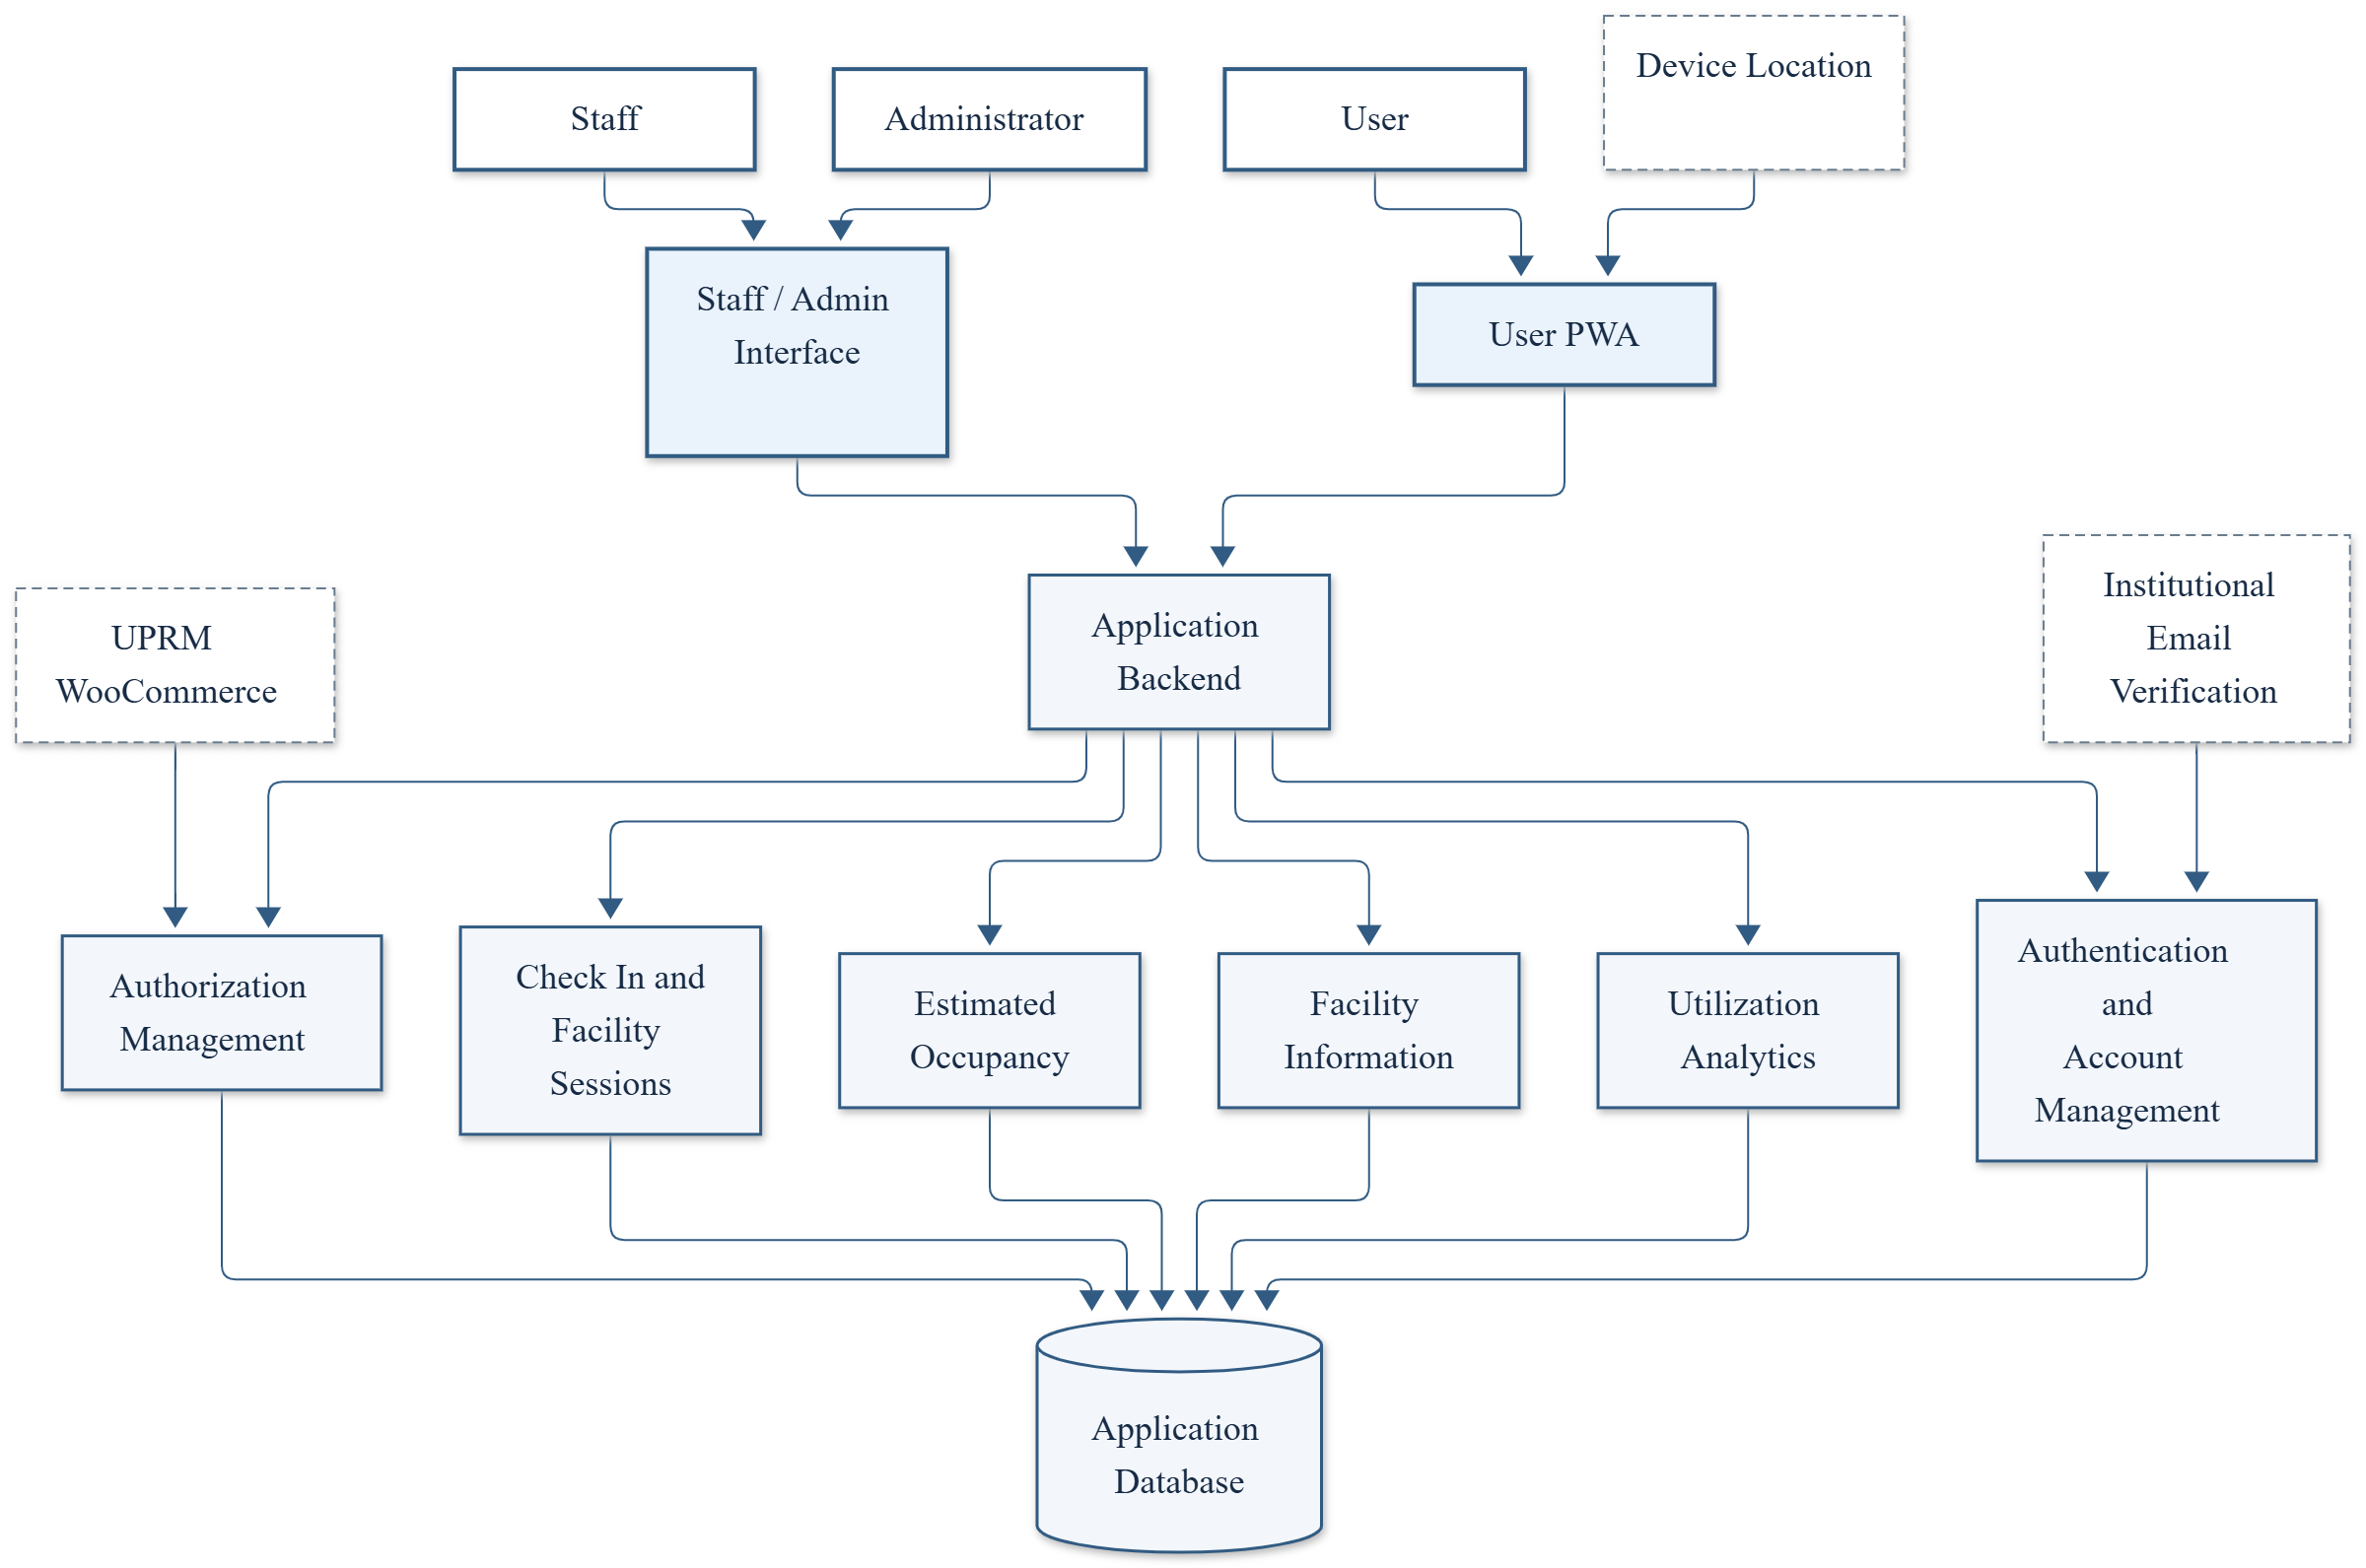
\includegraphics[width=0.98\textwidth,height=0.72\textheight,keepaspectratio]{diagrams/01_architecture.png}
\caption{High-Level System Architecture}
\label{fig:architecture}
\par\vspace{0.35em}\noindent\small\RaggedRight
Figure 1 shows how the User PWA and Staff/Administrator interface connect to the backend, its services, and the application database. WooCommerce, institutional email verification, and device location supply information to the relevant workflows.
\end{figure}

% --------------------------- FIGURE 2 ------------------------------
\begin{figure}[!htbp]
\centering
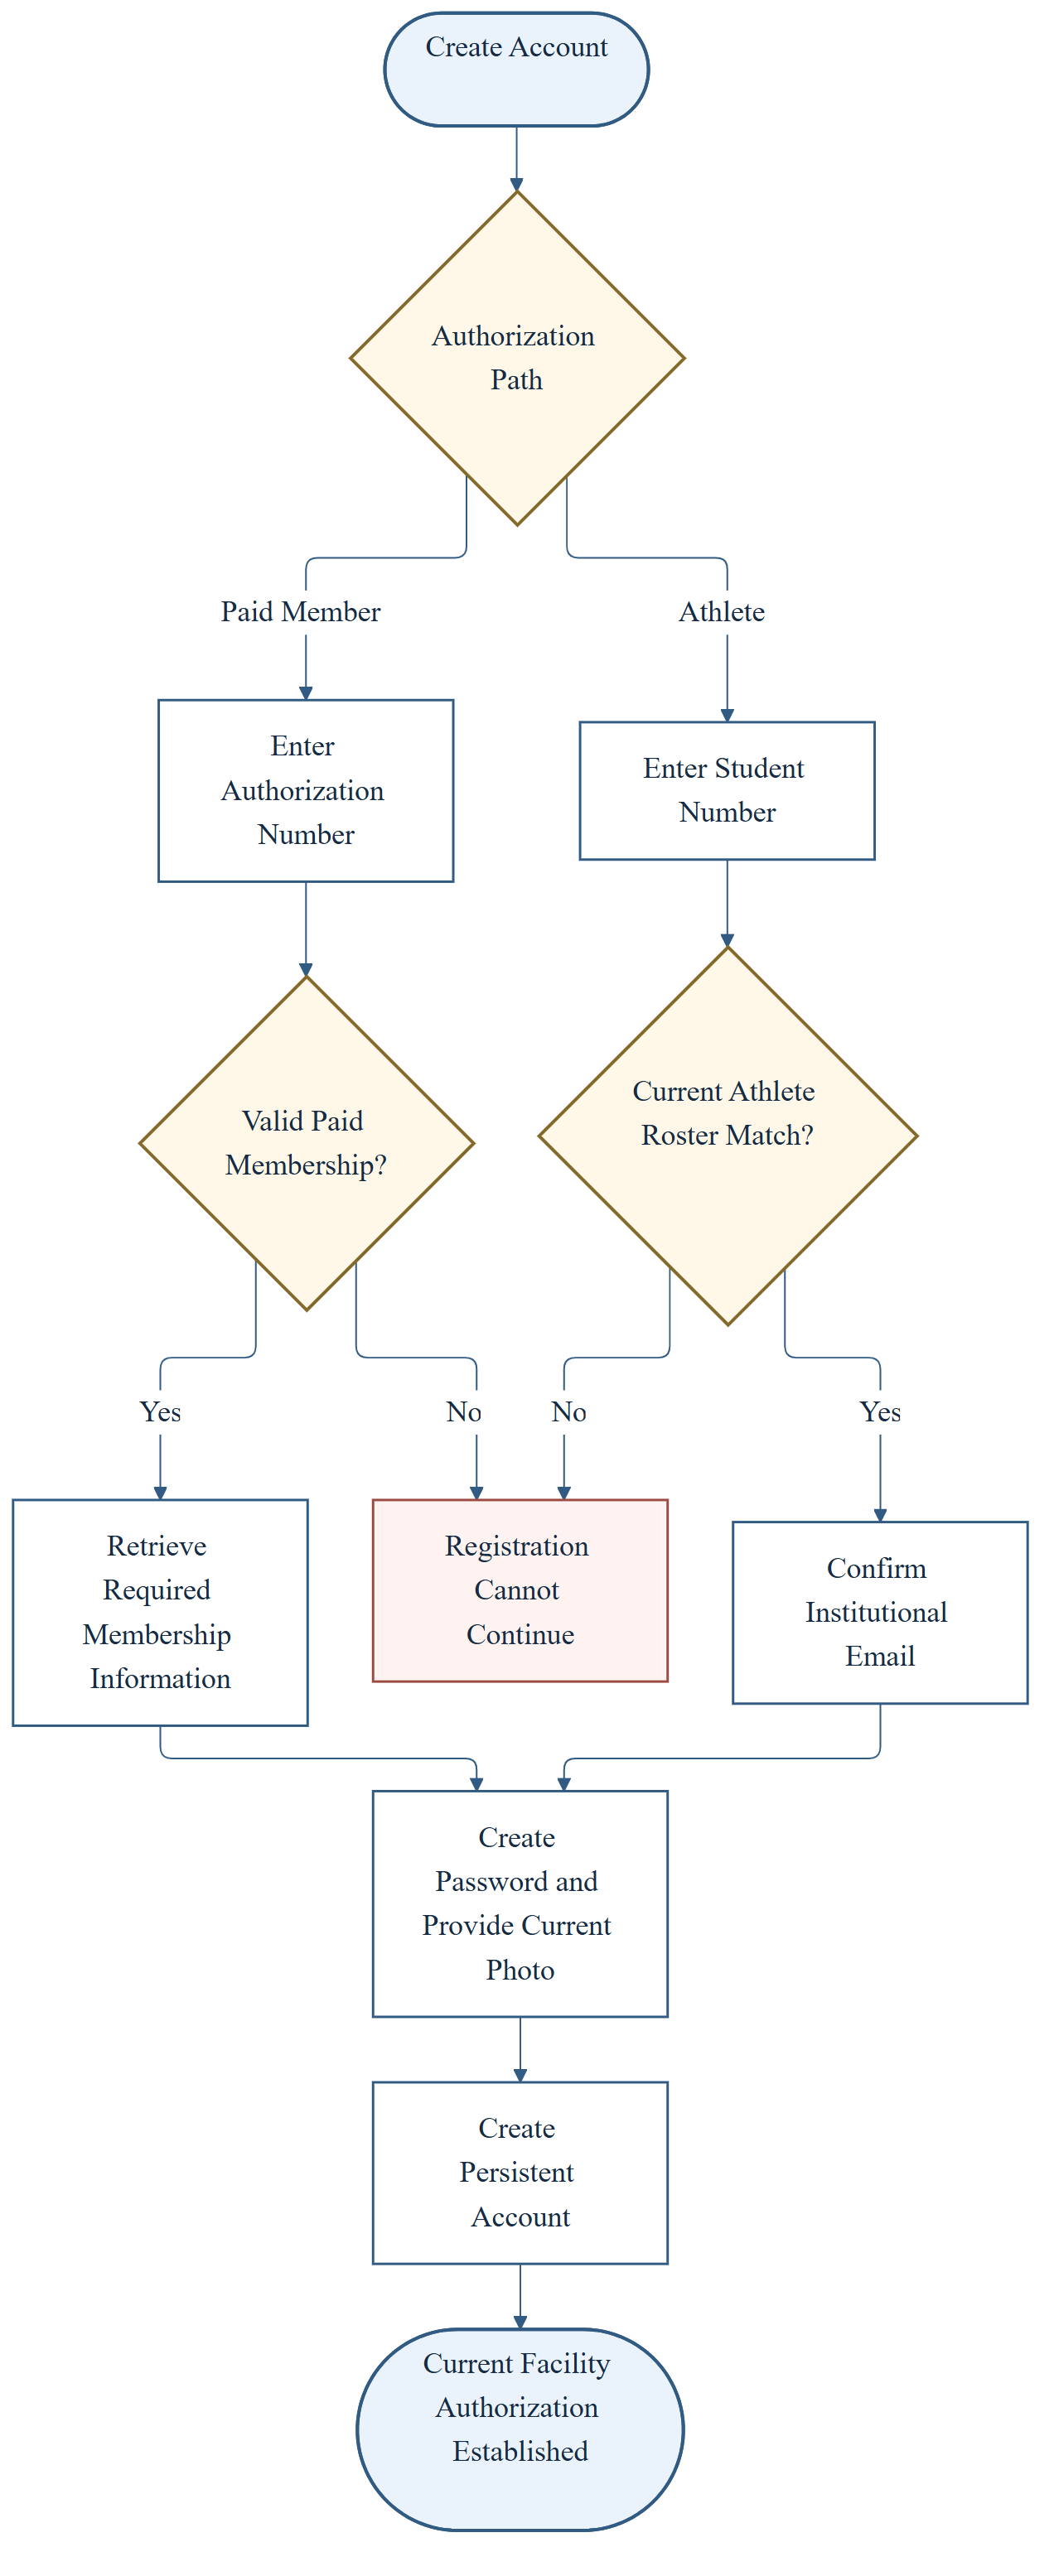
\includegraphics[width=0.98\textwidth,height=0.82\textheight,keepaspectratio]{diagrams/02_account_creation.png}
\caption{Paid-Member and Athlete Account Creation}
\label{fig:accountcreation}
\par\vspace{0.35em}\noindent\small\RaggedRight
Figure 2 separates paid-member validation by Authorization Number from athlete validation against the current roster. Both paths then create one persistent account with a password and current photo.
\end{figure}

% --------------------------- FIGURE 3 ------------------------------
\begin{figure}[!htbp]
\centering
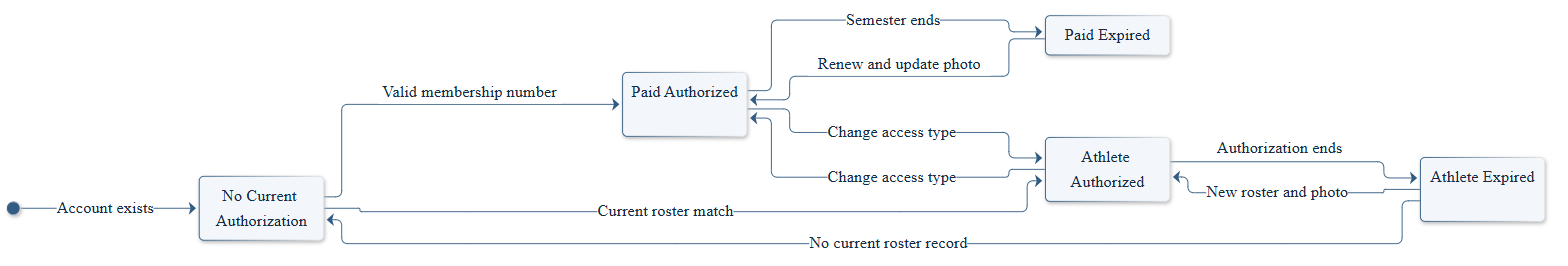
\includegraphics[width=0.98\textwidth,height=0.72\textheight,keepaspectratio]{diagrams/03_authorization_lifecycle.png}
\caption{Post-Registration Account and Authorization Lifecycle}
\label{fig:lifecycle}
\par\vspace{0.35em}\noindent\small\RaggedRight
Figure 3 begins after a persistent account has been established. Authorization may expire, be renewed, or change between paid-member and athlete access while the same User account remains intact.
\end{figure}

% --------------------------- FIGURE 4 ------------------------------
\begin{figure}[!htbp]
\centering
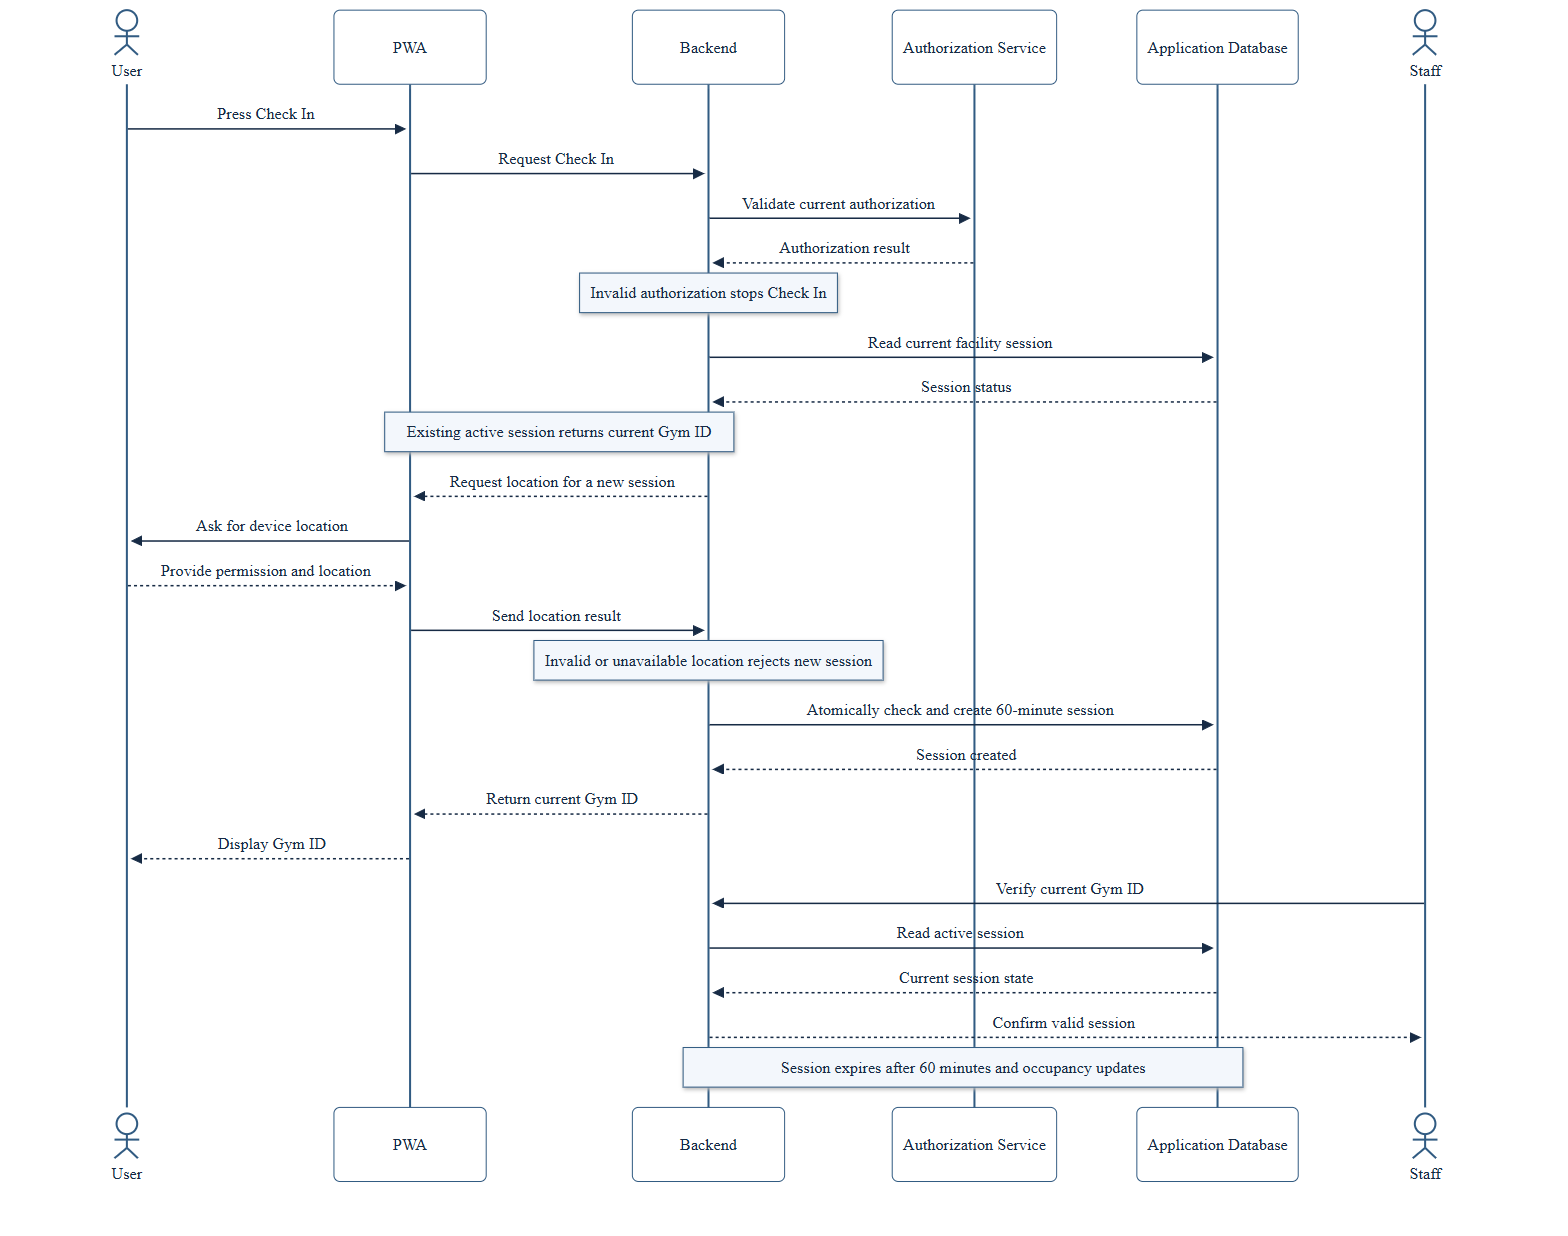
\includegraphics[width=0.98\textwidth,height=0.72\textheight,keepaspectratio]{diagrams/04_checkin_session.png}
\caption{Check-In and Facility Session Sequence}
\label{fig:checkin}
\par\vspace{0.35em}\noindent\small\RaggedRight
Figure 4 shows how authorization, location, active-session control, Gym ID, and Staff verification interact during Check In. The active-session check and session creation are handled as one protected backend operation so simultaneous requests cannot create overlapping sessions. Location is requested only when a new session is needed. A second Check In during an existing session returns the current Gym ID, while another valid Check In may create a new session after expiration. The notes identify rejection conditions without adding alternative branches to the sequence.
\end{figure}

% --------------------------- FIGURE 5 ------------------------------
\begin{figure}[!htbp]
\centering
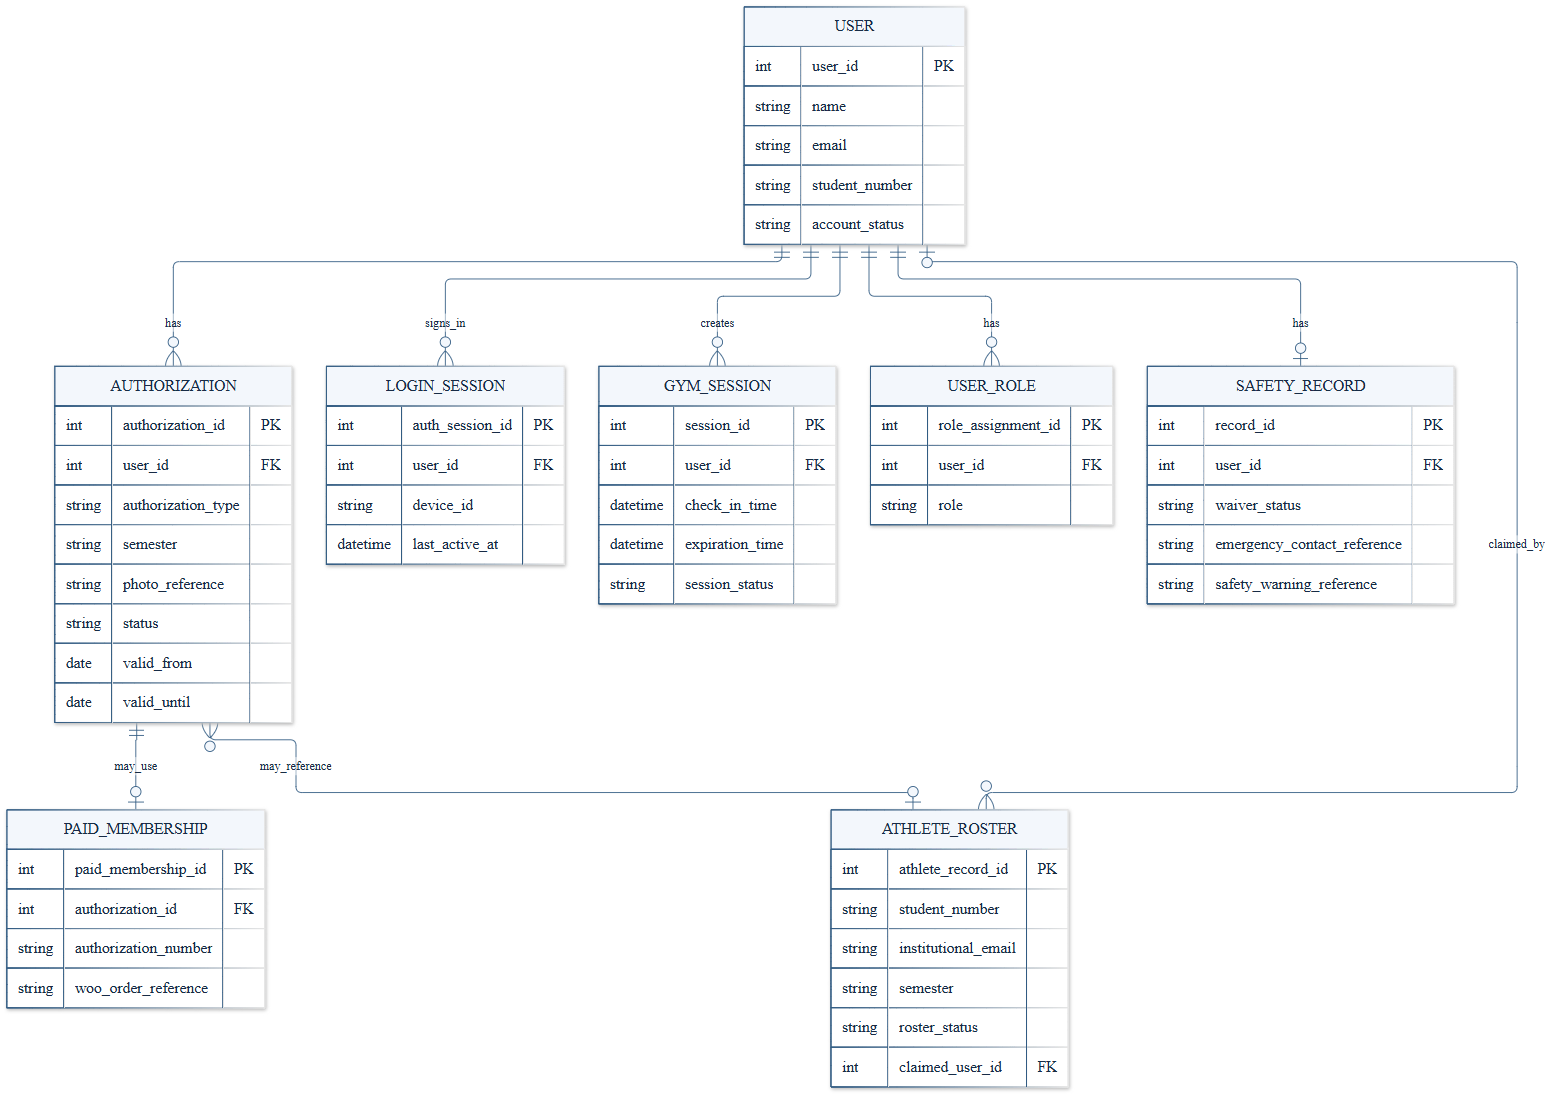
\includegraphics[width=0.98\textwidth,height=0.72\textheight,keepaspectratio]{diagrams/05_data_model.png}
\caption{Conceptual Data Model}
\label{fig:datamodel}
\par\vspace{0.35em}\noindent\small\RaggedRight
Figure 5 separates identity, authorization, login-session state, facility sessions, roles, and protected membership information. The model keeps semester-specific photographs with Authorization rather than treating the photograph as a permanent User attribute.

Facility schedules, rules, and equipment content are omitted so the diagram remains focused on identity, authorization, sessions, and protected membership records.
\end{figure}

\subsection{Related Works}

\textbf{Progressive Web Applications.} Królikowski and Miłosz studied factors that affect PWA performance on mobile devices, including resource minimization, lazy loading, and distributed content delivery. Their work informs the performance considerations for the selected PWA implementation rather than being the reason a PWA was chosen [3].

\textbf{Indoor smartphone location.} NIST evaluated smartphone location technologies across five large buildings and found measurable differences in indoor localization performance between Android and iPhone. This supports treating device location as supporting evidence for Check In rather than exact proof of presence, and supports setting the final location boundary and accepted accuracy through tests at the actual Weight Gym [4].

\textbf{Role-Based Access Control.} The NIST RBAC model describes authorization in terms of users, roles, and permissions rather than direct access to every resource. It informs the separation of User, Staff, and Administrator privileges and supports keeping Developer/Maintainer access outside normal gym operational roles [5].

These works influence three engineering decisions: PWA performance, treatment of indoor device location, and the access-control structure. They are technical foundations, not claims that the system is unique.

\subsection{Engineering Constraints and Verification}

\begin{center}
\small
\begin{longtable}{L{3.1cm} L{5.1cm} L{5.2cm}}
\toprule
\textbf{Constraint and reason} & \textbf{Engineering response} & \textbf{Pass condition / timing} \\
\midrule
\endfirsthead
\toprule
\textbf{Constraint and reason} & \textbf{Engineering response} & \textbf{Pass condition / timing} \\
\midrule
\endhead
\bottomrule
\endlastfoot
\textbf{WooCommerce source.} Membership data remains in an external system. & Keep WooCommerce authoritative, copy only needed fields, and use controlled imports so upstream changes do not redesign accounts. & Re-import produces no duplicate; corrected, refunded, or cancelled orders update authorization (Sprints 1--3). \\
\addlinespace
\textbf{Indoor location [4].} Phone accuracy varies by device and indoors. & Require a reading; compare gym boundary and reported accuracy; set the threshold through on-site tests. & Inside, outside, denied-permission, and low-accuracy cases pass on real phones at the gym (Sprints 4--5). \\
\addlinespace
\textbf{Connectivity.} Login, authorization, sessions, one-device enforcement, and Gym ID verification need the backend. & Require connectivity; disable offline Check In to avoid inconsistent access and occupancy. & Offline Sign In and Check In create no session (Sprints 4--5). \\
\addlinespace
\textbf{Concurrency.} Simultaneous requests can duplicate sessions or claims. & Enforce database uniqueness and atomic Check In, not frontend-only checks. & Concurrent requests and repeated Authorization Number or athlete-record claims yield one session or claim (Sprints 2--6). \\
\addlinespace
\textbf{Browser/device variation.} PWA and geolocation behavior vary. & Test real phones on iPhone/Safari and Android/Chrome; test Windows/Chrome and Edge, with secondary macOS/Firefox checks. & Core flows pass the defined device/browser matrix (Sprints 4--8, 11). \\
\addlinespace
\textbf{Sensitive data.} Photos, waivers, emergency contacts, and safety approvals need protection. & Restrict by role, use private storage and minimal collection, and define retention; Staff sees only Check In essentials. & Role-permission tests confirm least-needed record access (Sprints 7--8). \\
\addlinespace
\textbf{Prototype infrastructure.} Free-tier services are suitable for Capstone demonstration, not assumed production. & Reevaluate infrastructure before institutional deployment; keep recoverable copies. & Database and Storage exports restore before each milestone. \\
\end{longtable}
\end{center}

\subsection{Engineering Standards}

The project will apply standards that are directly connected to the technologies and risks of the platform. Standards are included only when they have a clear role in the implementation.

\begin{center}
\small
\begin{longtable}{L{3.6cm} L{4.4cm} L{5.6cm}}
\toprule
\textbf{Standard} & \textbf{Application to the Project} & \textbf{Justification} \\
\midrule
\endfirsthead
\toprule
\textbf{Standard} & \textbf{Application to the Project} & \textbf{Justification} \\
\midrule
\endhead
\bottomrule
\endlastfoot

WCAG 2.2 -- relevant Level AA criteria [6]
&
User, Staff, and Administrator web interfaces
&
Targets accessible forms, navigation, touch interactions, and status information. Key states such as the live Gym ID use text or icons in addition to color. \\
\addlinespace
\midrule
\addlinespace

W3C Geolocation specification [7]
&
Location-based Check In
&
Uses browser-provided geolocation through the standard API. Permission state and reported accuracy are handled in the Check In flow. \\
\end{longtable}
\end{center}

\subsection{Engineering Best Practices}

\textbf{Security and access.} Users receive only role-required access; Staff have no unrestricted administrative access, and Developers do not routinely access production safety or emergency data. Row Level Security and server-side checks protect exposed tables and privileged actions; credentials remain in protected server configuration.

\textbf{Integrity and privacy.} Database constraints prevent duplicate athlete-roster and paid Authorization Number claims and overlapping active sessions. Only needed WooCommerce fields are copied. Location is used for Check In, not stored as movement history; an audit may retain its validation result. Photos use protected storage; older photos are discarded unless UPRM requires retention.

\textbf{Reliability and recovery.} WooCommerce data is validated before granting access, and unverifiable records fail safely. Staff corrections, athlete-roster changes, and Staff-role assignments record actor, action, affected record, and timestamp. Before major milestones, code and schema are kept in Git and database and Storage exports are taken as needed.

\textbf{Development and testing.} Git branches and reviewed pull requests separate development from deployable main; reproducible migrations and separate development/deployed configuration control changes. Automated unit or database tests cover authorization and sessions; integration tests cover authentication through session creation; real devices verify location and PWA behavior. Testing Plan cases map to the measurable objectives.

%=====================================================================
\section{Project Plan}
%=====================================================================

\subsection{Activities and Process}

The team works in one-week Scrum sprints. At planning, it selects objective-linked backlog tasks, splitting oversized work; several weekly standups report progress, plans, and blockers. Blockers affecting the sprint are handled the same day, while others return to the backlog. Each sprint ends with an acceptance-criteria review and retrospective that revises the backlog and test plan. The five objectives generally proceed in dependency order, with independent later tasks pulled forward when practical; all three members contribute by layer.

\subsection{Timetable, Milestones, and Deliverables}

\begin{center}
\small
\begin{longtable}{L{1.4cm} L{2.3cm} L{5.4cm} L{4.5cm}}
\toprule
\textbf{Sprints} & \textbf{Dates} & \textbf{Work} & \textbf{Milestone and deliverable} \\
\midrule
\endfirsthead
\toprule
\textbf{Sprints} & \textbf{Dates} & \textbf{Work} & \textbf{Milestone and deliverable} \\
\midrule
\endhead
\bottomrule
\endlastfoot
1--3 & Sep 30--Oct 20 & Repository, environment, schema, WooCommerce export, paid and athlete authorization, account creation, and controlled fixes. & Oct 16: validated identity and authorization workflow (Objective 1). \\
\addlinespace
4--5 & Oct 21--Nov 3 & Check In UI, geolocation and boundary checks, atomic creation, expiration, duplicate handling, Gym ID, and scenario tests. & Oct 30: tested 60-minute Check In and session flow (Objective 2). \\
\addlinespace
6 & Nov 4--10 & Occupancy calculation, interface consistency, and controlled tests. & Nov 6: verified shared occupancy estimate (Objective 3). \\
\addlinespace
7--8 & Nov 11--24 & Staff dashboard, Administrator tools, role matrix, and fixes. & Nov 20: tested role-controlled operational tools (Objective 4). \\
\addlinespace
9--10 & Nov 25--Dec 8 & Utilization calculations by period, high/low use, and authorization type; analytics view and tests. & Dec 4: validated analytics and Administrator view (Objective 5). \\
\addlinespace
11 & Dec 9--16 & Integrated end-to-end testing, documentation, and submission. & Dec 16: final integrated prototype and documentation. \\
\end{longtable}
\end{center}

\subsection{Team Responsibilities}

\begin{center}
\small
\begin{tabularx}{0.95\textwidth}{L{3.4cm} X}
\toprule
\textbf{Member / focus} & \textbf{Specific tasks} \\
\midrule
Team Member 1 / Backend and data model & Design PostgreSQL users, authorizations, terms, roster, sessions, and roles; implement paid/athlete verification and Row Level Security; enforce atomic Check In, 60-minute expiration, active-session occupancy, and Staff/Administrator backend permissions. \\
\addlinespace
Team Member 2 / Frontend and PWA & Build account creation, Sign In, and renewal; geolocation Check In and Gym ID; user occupancy and facility pages; Staff/Administrator dashboards; responsive behavior across the device/browser matrix. \\
\addlinespace
Team Member 3 / Integration, analytics, and testing & Build WooCommerce import and reconciliation; calculate period, peak/low-use, and authorization-type analytics; maintain controlled datasets; coordinate sprint regression and device/location tests; track blockers to resolution or backlog placement. \\
\bottomrule
\end{tabularx}
\end{center}

\subsection{Testing Plan}

Tests run as sprint backlog items are completed. \textbf{Authorization (Sprints 1--3):} a controlled dataset checks valid/expired paid memberships, valid/invalid athlete approvals, missing authorization, and unmatched users against expected approve/deny decisions. \textbf{Check In and sessions (Sprints 4--5):} tests cover location inside/outside the boundary, denied permission, inadequate accuracy, successful/rejected and duplicate Check Ins, automatic expiration, and concurrent requests that must create at most one session. Staff-assisted Check In tests verify the authorized user without a smartphone, photo and authorization checks, actor/timestamp audit, and no overlapping session.

\textbf{Occupancy (Sprint 6):} expected active-session counts are compared after Check Ins, expirations, Staff corrections, and concurrent events; User, Staff, and Administrator views must agree. \textbf{Roles (Sprints 7--8):} the permission matrix confirms allowed actions succeed and forbidden actions fail. \textbf{Analytics (Sprints 9--10):} each finalized metric is compared with a known result from controlled historical data. Tests from prior work rerun at each sprint start; Sprint 11 checks all five areas together against one integrated dataset from Check In to analytics. Engineering-constraint pass conditions and timing appear in Engineering Constraints and Verification.

%=====================================================================
\section{Previous Work and References}
%=====================================================================

\begingroup\sloppy
\begin{enumerate}[label={[\arabic*]},leftmargin=2.2em,itemsep=6pt]

\item GymMaster, ``All-In-One Gym Management Software.'' [Online]. Available: \url{https://www.gymmaster.com/business/gym-software/}. Accessed: Sep. 29, 2026.

\item TeamUp, ``Access Control Software.'' [Online]. Available: \url{https://goteamup.com/features/access-control}. Accessed: Sep. 29, 2026.

\item J. Królikowski and M. Miłosz, ``Study of factors affecting the performance of web applications on mobile devices,'' \textit{Journal of Computer Sciences Institute}, vol. 36, pp. 271--277, 2025, doi: 10.35784/jcsi.7430.

\item N. Moayeri, C. Li, and L. Shi, ``Indoor Localization Accuracy of Major Smartphone Location Apps,'' in \textit{Proc. IEEE Wireless Communications and Networking Conference (WCNC)}, Marrakech, Morocco, 2019, doi: 10.1109/WCNC.2019.8885639.

\item R. Sandhu, D. F. Ferraiolo, and D. R. Kuhn, ``The NIST Model for Role-Based Access Control: Towards a Unified Standard,'' in \textit{Proc. Fifth ACM Workshop on Role-Based Access Control}, Berlin, Germany, pp. 47--63, 2000, doi: 10.1145/344287.344301.

\item World Wide Web Consortium (W3C), ``Web Content Accessibility Guidelines (WCAG) 2.2,'' W3C Recommendation, Dec. 12, 2024. [Online]. Available: \url{https://www.w3.org/TR/WCAG22/}. Accessed: Sep. 29, 2026.

\item World Wide Web Consortium (W3C), ``Geolocation.'' [Online]. Available: \url{https://www.w3.org/TR/geolocation/}. Accessed: Sep. 29, 2026.

\end{enumerate}
\endgroup

\end{document}